Comme présenté en section \ref{subsec:architectureBefore} (page~\pageref{subsec:architectureBefore}), l'application \textit{symbolist} possède certains problèmes dans son architecture logicielle. Aussi, une des activités de ce stage a été de remédier à la structure de l'application \textit{symbolist} en lui appliquant le design pattern \textit{Model-View-Controller}, avec quelques adaptations de circonstances.
La présente section rend compte des changements appliqués à l'architecture de \textit{symbolist}, dans une démarche de stabilisation structurelle.

\subsection{Application du design pattern Model-View-Controller}
\label{subsec:applicationDuMVC}
Le \og paradigme \fg \textit{MVC} est une manière de structurer une application qui relève d'une séparation en trois parties : le modèle, la vue et le contrôleur \cite{krasner1988}. Le but de la manœuvre est de confiner les préoccupations fonctionnelles de chaque partie, et de définir leurs interactions afin de rendre plus intuitive la marche à suivre par le programmeur lors de l'implémentation d'une nouvelle fonctionnalité.

\paragraph{Implémentation de la structure élémentaire} Le framework \textit{JUCE} ne disposant pas de classes abstraites décrivant les parties du \textit{MVC}, la structure sous-jacente de l'architecture a été implémentée en \textit{C++}. La figure \ref{fig:mvcApi} décrit le diagramme de classes définissant les concepts élémentaires de l'architecture \textit{MVC}. Ce diagramme a servi de base pour l'implémentation de la structure \textit{MVC} dans \textit{symbolist}.

\begin{figure}[H]
	\centering
	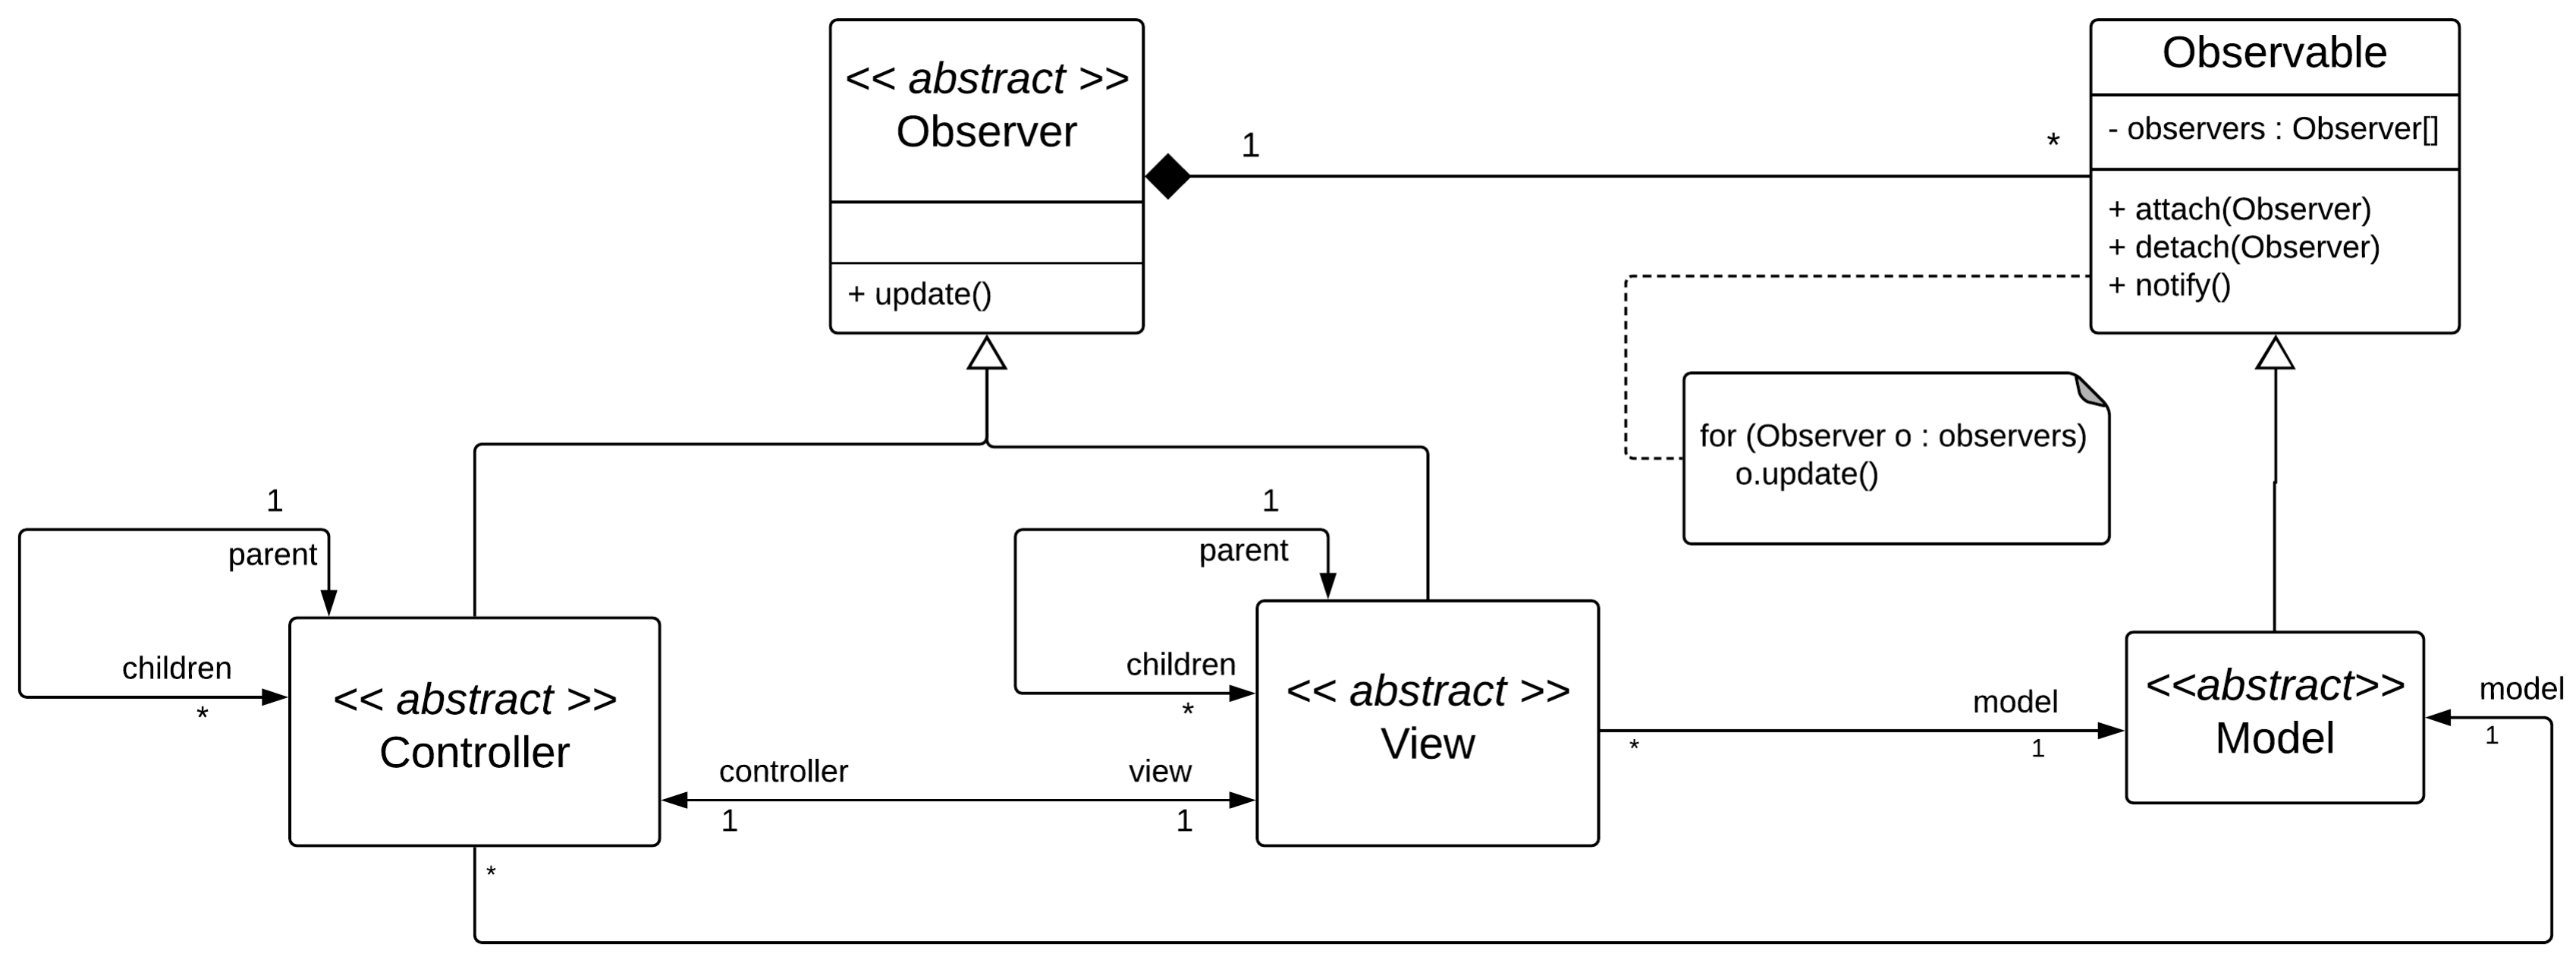
\includegraphics[keepaspectratio=true, width=\textwidth]{ArchitectureLogicielleSymbolist/i/mvcApi.png}
	\caption{Diagramme de classes pour une API MVC}
	\label{fig:mvcApi}
	\small
	\it
\end{figure}

Premièrement, dans le paradigme \textit{MVC}, les vues et les contrôleurs de l'application sont informés des changements survenus dans le modèle par le biais d'un système de souscription, plus connu sous le nom de design pattern \textit{Observer}. Comme présenté en figure \ref{fig:mvcApi}, les contrôleurs et vues du système héritent de la classe \textit{Observer} la méthode \textit{update}, qui est appelé par l'objet observé, ici le modèle héritant de la classe \textit{Observable}, lorsque celui-ci est modifié.
Toutes actions d'écriture dans le modèle déclenche l'envoi du message \textit{update} aux observateurs. Par exemple, dans le cas de \textit{symbolist}, la création ou la délétion d'un symbole dans la partition ou dans la palette donne lieu à l'envoi du message \textit{update}.
La réaction des observateurs à la réception du message \textit{update} doit être définie dans les sous-classes de la classe \textit{Observer}. Aussi, les classes \textit{Controller} et \textit{View} décrivant des comportements génériques pour les vues et contrôleurs d'une application, aucune implémentation de la méthode \textit{update} n'y est définie, d'où leur statut de classe abstraite.

Deuxièmement, les relations entre les classes \textit{Controller}, \textit{View} et \textit{Model} sont définis comme présentées en figure \ref{fig:mvcApi}. Un contrôleur et une vue sont associés par couple; ils se référencent mutuellement. Chaque vue et chaque contrôleur d'une application connaissent le modèle auquel ils sont rattachés; ils en ont un accès direct. Cependant, le modèle d'une application ne connaît pas directement les contrôleurs et les vues qui l'observent; il les contacte par le biais du message \textit{update} exclusivement.

Troisièmement, l'interface d'une application pouvant être découpée en sous-vues, un système de hiérarchie a été mis en place, représentée par les relations réflexives des classes \textit{View} et \textit{Controller}. En effet, dans le paradigme \textit{MVC}, la hiérarchie des vues est répliquée pour les contrôleurs \cite{krasner1988}. Aussi, une application sera composée d'une vue \textit{racine}, la fenêtre du programme, laquelle sera divisée en sous-vues. Parallèlement, cette application possèdera un contrôleur \textit{racine} associé à la vue \textit{racine}, qui sera le parent de sous-contrôleurs associés à chaque sous-vues du programmes.

\paragraph{Structures préexistantes} La structure du programme \textit{symbolist} avant restructuration a été présentée succinctement en section \ref{subsec:architectureBefore} (page~\pageref{subsec:architectureBefore}). Le modèle de l'application étant détaillé en annexe \ref{sec:symbolistModelClassDiagram}, page~\pageref{sec:symbolistModelClassDiagram}, seules les parties vue et contrôleur de l'application seront présentées ici.
La figure \ref{fig:controllerDiagramBefore} décrit le diagramme de classes \og côté contrôleur \fg, au début du stage.

\begin{figure}[H]
	\centering
	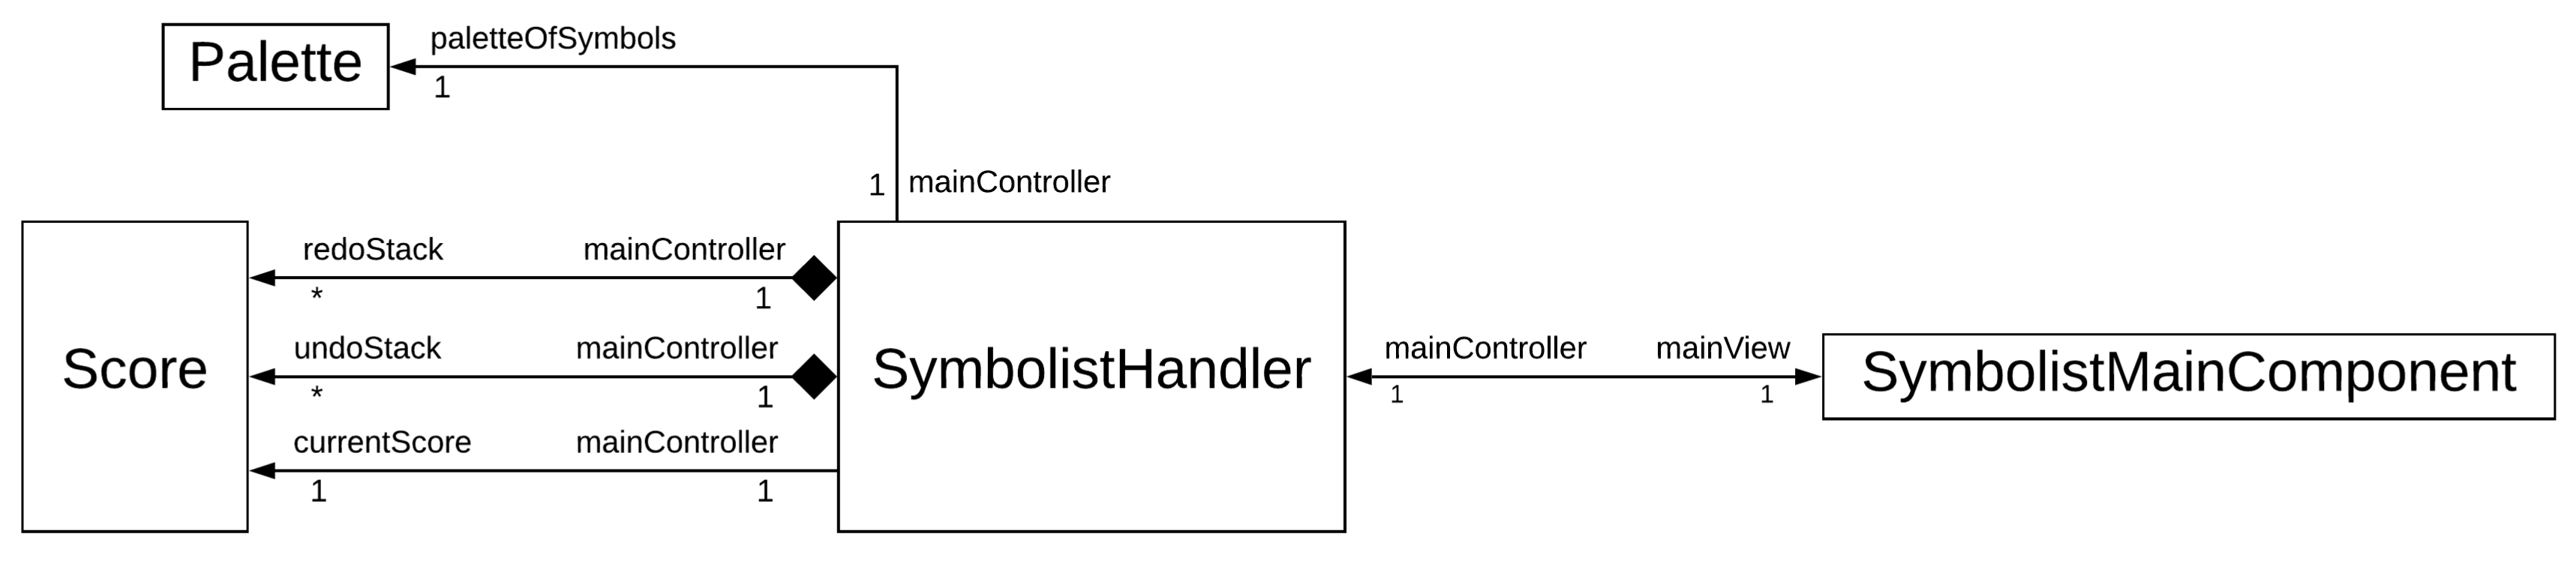
\includegraphics[keepaspectratio=true, width=\textwidth]{ArchitectureLogicielleSymbolist/i/controllerDiagramBefore.png}
	\caption{Diagramme de classes pour la partie contrôleur avant restructuration}
	\label{fig:controllerDiagramBefore}
	\small
	\it
\end{figure}

Avant restructuration, la classe \textit{SymbolistHandler} est la seule à référencer directement le modèle, représenté par les classes \textit{Palette} et \textit{Score}. Les vues de l'application doivent systématiquement passer par la classe \textit{SymbolistHandler} afin d'accéder aux données du modèle. Préliminairement à la restructuration, le couple contrôleur principal-vue principale est déjà réifié par la liaison entre la classe \textit{SymbolistHandler} et \textit{SymbolistMainComponent}.

La figure \ref{fig:viewDiagramBefore} expose le diagramme de classes simplifié de la partie \og vue \fg de l'application \textit{symbolist} au début du stage.

\begin{figure}[H]
	\centering
	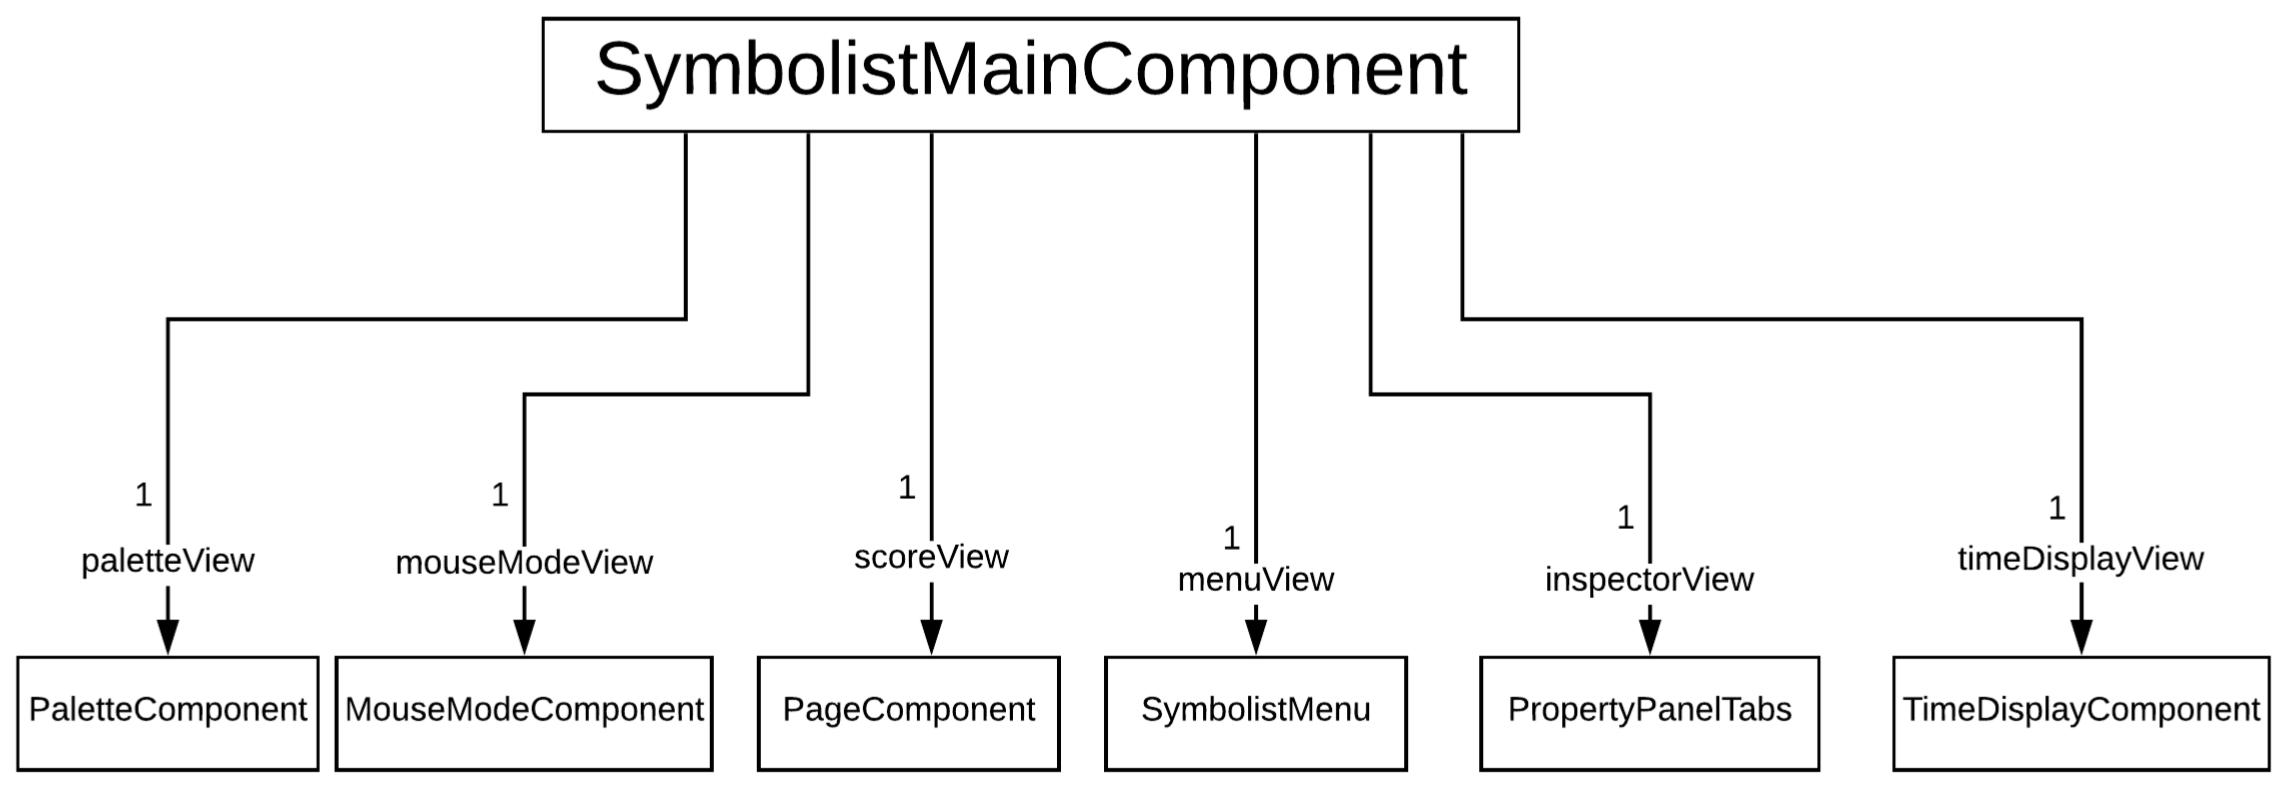
\includegraphics[keepaspectratio=true, width=0.8\textwidth]{ArchitectureLogicielleSymbolist/i/viewDiagramBefore.png}
	\caption{Diagramme de classes pour la partie vue avant restructuration}
	\label{fig:viewDiagramBefore}
	\small
	\it
\end{figure}

La classe \textit{SymbolistMainComponent} représente la vue principale de l'application \textit{symbolist}. Elle référence toutes les sous-vues de l'application, comme la vue représentant la palette des symboles utilisables (\textit{paletteView}) et la vue décrivant la partition (\textit{scoreView}).

\paragraph{Implémentation du design pattern MVC} La première démarche de restructuration a été de faire hériter les classes de l'application \textit{symbolist} des classes de l'API \textit{MVC} présentées un peu avant.
La classe \textit{SymbolistHandler} a donc hérité de la classe \textit{Controller} et la classe \textit{SymbolistMainComponent} et ses sous-vues ont hérité de la classe \textit{View}.
Afin de lier chaque instance de \textit{View} et \textit{Controller} à une instance du modèle, une classe \textit{SymbolistModel} a été créée, référençant la partition et la palette de l'application.
L'encapsulation des classes \textit{Score} et \textit{Palette} dans \textit{SymbolistModel} permet d'envoyer plus facilement le message \textit{update} aux observateurs du modèle à chaque fois qu'une action de modification est entreprise.

Ensuite, un contrôleur a été créé et couplé avec chacune des sous-vues de l'application afin de gérer plus localement les interactions avec l'utilisateur.  
Une fois la structure globale de l'application établie, le travail a consisté à s'assurer que les éléments de l'architecture MVC se comportent correctement, depuis la captation d'une action utilisateur jusqu'à sa répercussion sur l'interface graphique de \textit{symbolist}.
Pour plus d'informations sur la structure finale du programme, le diagramme de classes décrivant la nouvelle architecture de l'application \textit{symbolist} est présentée en annexe \ref{sec:symbolistFinalStructure}, page~\pageref{sec:symbolistFinalStructure}.

\subsection{Restructuration de la hiérarchie des composants graphiques}
\label{susec:graphicComponentRestruct}
Une des volontés de \textit{symbolist} est de conserver l'information descriptive des symboles de la partition dans le canevas d'un bundle OSC. De fait, le modèle de l'application \textit{symbolist} ne possède qu'une seule classe \textit{Symbol} pour décrire les éléments d'une partition.
La structure hiérarchique (encapsulation de symboles dans d'autres symboles) qui peut être celle d'une partition \textit{symbolist} se trouve cachée dans les bundles OSC du modèle.
Aussi, ce sont aux classes représentant graphiquement les symboles de refléter cette structure.
De même, si les symboles du modèle participent d'une seule et même classe \textit{Symbol}, il possède cependant un attribut \textit{type} qui va orienté le contenu des messages OSC composant le bundle les décrivant.
Par exemple, un symbole de type \textit{circle} possédera l'attribut \textit{radius} dans son bundle, alors qu'un symbole de type \textit{rectangle} possèdera un attribut \textit{width} et \textit{height}.
Au même titre que chaque type de symbole oriente la construction du bundle sous-jacent, les classes à composants graphiques décrivant la partition \textit{symbolist} doivent être spécialisées pour refléter chacun des types de symboles.
Au début de ce stage, la hiérarchie des composants graphiques est déjà établie. La figure \ref{fig:graphicCompBefore} présente la diagramme de classes, avant restructuration, des composants décrivant une partition \textit{symbolist}.

\begin{figure}[H]
	\centering
	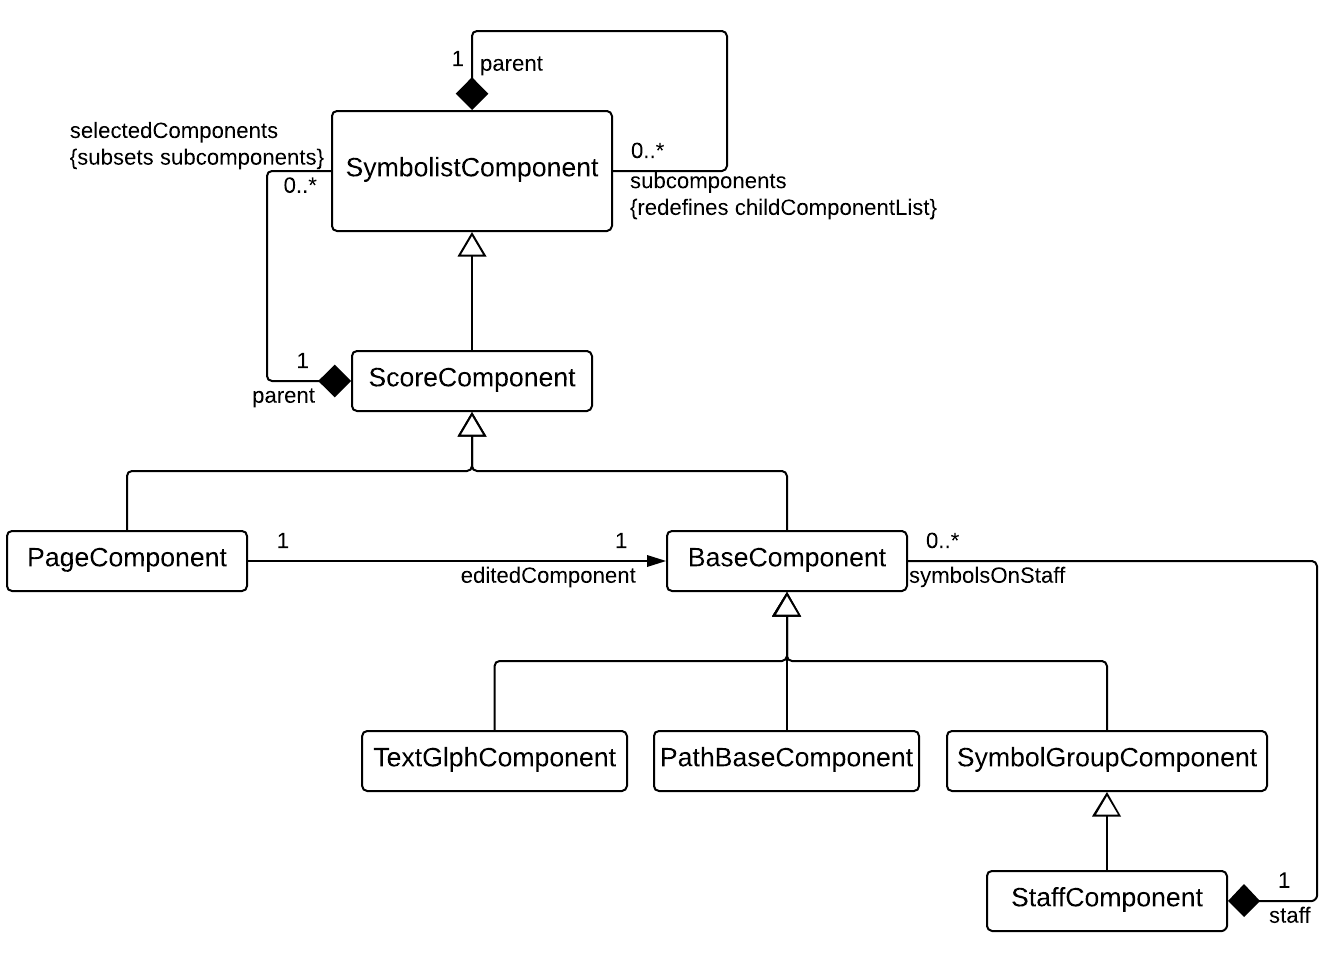
\includegraphics[keepaspectratio=true, width=0.8\textwidth]{ArchitectureLogicielleSymbolist/i/graphicCompBefore.png}
	\caption{Diagramme de classes des composants graphiques d'une partition symbolist avant restructuration}
	\label{fig:graphicCompBefore}
	\small
	\it
	La classe \emph{SymbolistComponent} est la classe mère de tous les composants graphiques de l'application \emph{symbolist}. Elle contient des méthodes de récupération de référence vers les vues principales, comme \emph{SymbolistMainComponent}, et vers la classe \emph{SymbolistHandler}.
	La classe \emph{ScoreComponent} est la classe mère de tous les composants graphiques appartenant à une partition \emph{symbolist}.
	La classe \emph{PageComponent} correspond à la vue de la partition, elle est associée à un \emph{PageController}.
	La classe \emph{BaseComponent} et ses sous-classes décrivent plus précisément chaque type de symbole graphique de la partition, qu'ils soient dessinés par tracé (\emph{PathBaseComponent}), qu'ils représentent du texte (\emph{TextGlphComponent}) ou qu'ils soient une composition de symboles
	(SymbolGroupComponent).
\end{figure}

La construction des classes comme présentéee en figure \ref{fig:graphicCompBefore} souffrent de quelques faiblesses structurelles. Par exemple, le design pattern \textit{Composite}, qui serait prescrit pour représenter la hiérarchie des composants graphiques, n'est que partiellement appliqué.
La classe \textit{PageComponent}, qui représente la partition et qui est donc un ultime groupe de symboles, n'est pas regroupée avec la classe \textit{SymbolGroupComponent} sous une même égide d'éléments composites.
De plus, la classe \textit{BaseComponent}, dont héritent tous les composants graphiques présents dans la partition, ne suffit pas à clairement différencier les éléments composites des éléments simples.

La structure globale des composants graphiques a été remaniée en conséquence. Le résultat du remaniement est présenté par le diagramme de classes de la figure \ref{fig:graphicCompAfter}.

\begin{figure}[H]
	\centering
	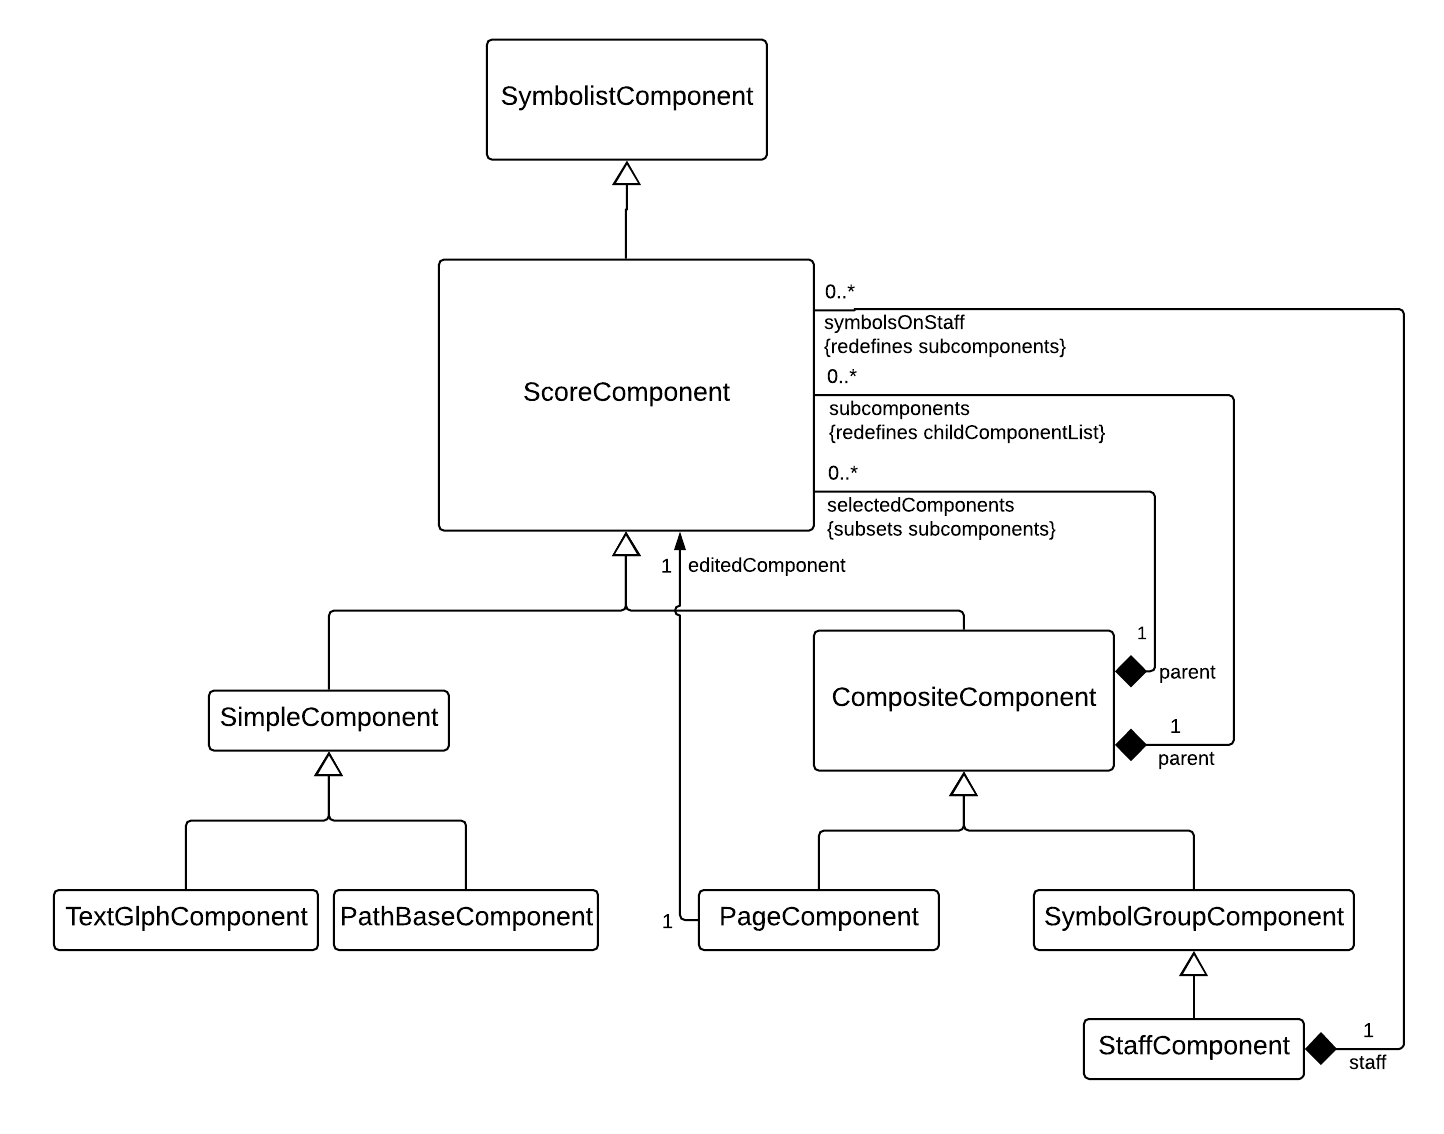
\includegraphics[keepaspectratio=true, width=0.8\textwidth]{ArchitectureLogicielleSymbolist/i/graphicCompAfter.png}
	\caption{Diagramme de classes des composants graphiques d'une partition symbolist après restructuration}
	\label{fig:graphicCompAfter}
	\small
	\it
\end{figure}

Deux nouvelles classes ont donc été crées pour appliquer pleinement le pattern \textit{Composite}: \textit{SimpleComponent} et \textit{CompositeComponent}\footnote{\textit{SymbolGroupComponent} aurait pu généraliser le concept d'élément composite, cependant cette classe étant concrète, une nouvelle classe abstraite \textit{CompositeComponent} a été créée.}. La classe \textit{PageComponent} a été déplacée pour hériter de la classe \textit{CompositeComponent}.
De même, les relations \textit{subcomponents}, \textit{symbolsOnStaff} et \textit{selectedComponents}, permettant la composition et la sélection de symboles dans les éléments composites ont migrés à leur juste place entre la classe \textit{CompositeComponent} et \textit{ScoreComponent}.

